%!TEX root = ../Thesis.tex
\chapter{Background}
\label{chap:background}
\section{Job scheduler}
This Chapter briefly overviews the well-known open-source workload manager we use at CSC -- IT Center for Science, Slurm \cite{10.1007/10968987_3}.

Let's first start with some definitions:

\begin{enumerate}
    \item \textbf{Resource Manager} is a software component for overseeing the resources within a cluster, typically under the control of a scheduler. Its responsibilities include:

    \begin{itemize}
        \item Management of various resources such as nodes, CPUs, GPUs, memory, and network.
        \item Coordination of job execution across compute nodes to ensure efficient resource utilization.
        \item Prevention of resource overlap among concurrent jobs.
    \end{itemize}
    \item \textbf{Scheduler} is a software module that manages user jobs within a cluster based on predefined policies. It interacts with users to receive and handle new jobs while controlling the Resource Manager. Key features of a Scheduler include:

    \begin{itemize}
        \item Provision of partitions, queues, and Quality of Service (QoS) settings to enforce policies and limits on job execution.
        \item Implementation of scheduling mechanisms such as backfilling, first-in-first-out (FIFO), etc.
        \item Provision of interfaces for defining job workflows (e.g., job scripts), specifying job dependencies, and issuing commands for job management (e.g., submission, cancellation, etc.).
    \end{itemize}

    \item \textbf{Batch-System} or \textbf{Workload Manager} is the combination of a scheduler and a resource manager, combining the features of both components to manage workload within the cluster efficiently.
\end{enumerate}

% Slurm is vital in orchestrating parallel computing environments, bridging the gap between users and computational resources. At its core, Slurm embodies the roles of a resource manager and a job scheduler. The resource manager is the key, facilitating the execution of parallel jobs across distributed computing nodes. In contrast, the job scheduler dynamically allocates and manages resources to efficiently handle a queue of pending tasks, employing sophisticated scheduling algorithms optimized for various criteria such as network topology, fair-share scheduling, and advanced reservations.

Slurm, initially known as the Simple Linux Utility for Resource Management, emerged in 2002 at Lawrence Livermore National Laboratory as a batch system tailored for Linux clusters. As HPC environments require sophisticated workload managers to efficiently manage and allocate computing resources among multiple users and tasks, it evolved into a sophisticated scheduling framework incorporating advanced plugins.

% Today, Slurm is a robust system. Renowned for its scalability, It has been deployed on most of the world's largest computing systems, catering to diverse computational needs across various domains.

% Designed with scalability in mind, Slurm prides itself on its ability to manage colossal systems. As an open-source software under the GPLv2 (GNU General Public License version 2), Slurm promotes accessibility and fosters an active global development community. Its system administrator-friendly interface, coupled with its emphasis on security and fault tolerance, renders it a favored choice among administrators.

The architecture of Slurm is modular and extensible, with many plugins available to cater to diverse requirements. At the core of Slurm, we have mainly the following three components:

\begin{itemize}
    \item \textbf{Slurmctld} serves as the central management daemon within the Slurm framework, orchestrating the activities of all other Slurm daemons and resources. Its primary functions include the monitoring of system resources and the allocation of these resources to incoming workloads (jobs). Additionally, Slurmctld is a connecting point for accepting and processing job submissions, ensuring efficient utilization of available computing resources.
    \item \textbf{Slurmdbd} offers a secure and centralized interface to interact with the database system, specifically tailored to cater to the needs of Slurm. This daemon enables features such as archiving accounting records and storing essential metadata related to job executions. It ensures the integrity and confidentiality of data while providing seamless access to critical information for administrative and analytical purposes.
    \item \textbf{Slurmd} functions as the compute node daemon, operating at the node level to oversee the execution of computational tasks. Among its key responsibilities, slurmd actively monitors the status of tasks running on the compute nodes, facilitating efficient task management and resource allocation. It also acts as a connecting point for receiving task assignments, launching tasks onto the compute nodes, and terminating tasks as per system requirements or user requests.
\end{itemize}

% In addition to the three main components mentioned above, Figure \ref{fig_slurm_overview} shows the general slum architecture. Users interact with Slurm using commands available in the login node.

% These plugins, from network topologies to authentication mechanisms, offer a customizable framework adaptable to different computing environments. Moreover, Slurm's robust plugin design allows for seamless integration of custom functionalities, empowering users to tailor the system to their specific needs.

% \begin{figure}[H]
%     \centering
%     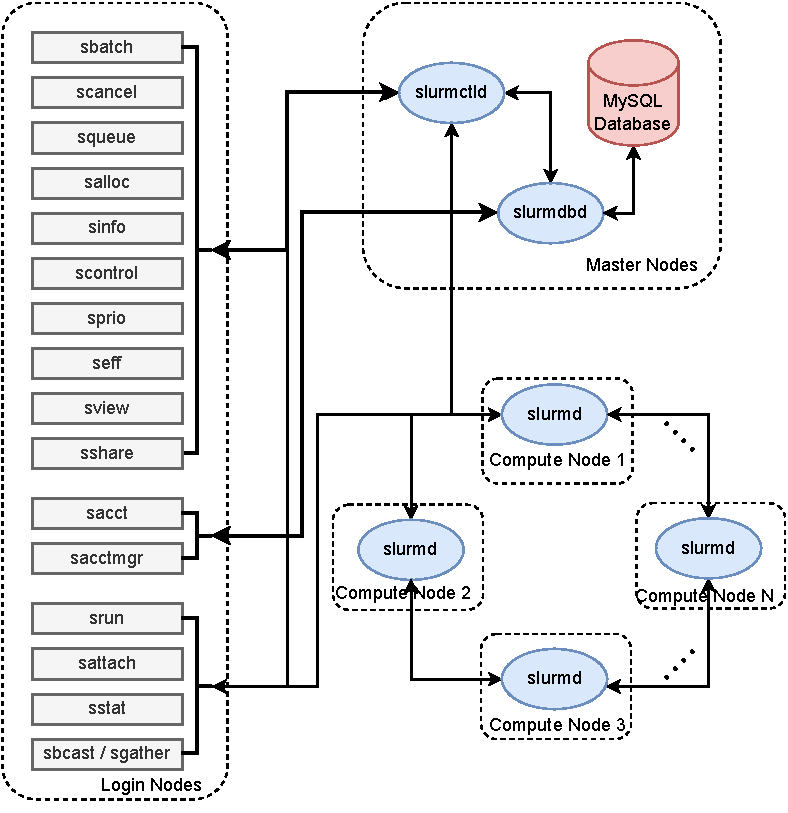
\includegraphics[width=0.8\textwidth]{figures/slurm-overview.pdf}
%     \caption{Slurm architecture overview}
%     \label{fig_slurm_overview}
% \end{figure}

% \begin{itemize}

%     \item \textbf{sbatch}: For submitting batch scripts, which can be written in bash, Perl, or Python, enabling users to automate the execution of tasks in a batch mode.
%     \item \textbf{scancel}: Enabling the cancellation of pending or running jobs or job steps, providing users with control over job management and resource allocation.
%     \item \textbf{squeue}: For querying pending and running jobs, providing users with visibility into the status of their submitted tasks and overall system workload.
%     \item \textbf{salloc}: For requesting interactive job allocations, users can access computing resources for their tasks interactively.
%     \item \textbf{sinfo}: Retrieving comprehensive information about partitions, reservations, and the state of nodes within the system, aiding users in understanding the availability and status of computing resources.
%     \item \textbf{scontrol}: Providing users with functionalities for managing jobs, querying system configurations, and retrieving resource utilization and allocation information.
%     \item \textbf{sprio}: Enabling users to query job priorities, assisting in resource allocation decisions and prioritization of tasks based on predefined criteria.
%     \item \textbf{seff}: Providing a concise overview of resource utilization for both active and completed batch jobs, detailing the requested and actual usage of resources.
%     \item \textbf{sview}: GUI that offers state information for jobs, partitions, and nodes, enhancing user experience in monitoring and managing computing resources.
%     \item \textbf{sshare}: Providing users with fair-share information, offering insights into resource allocation fairness among different users based on usage history and system policies.
%     \item \textbf{sacct}: Retrieving accounting information about jobs and job steps stored in Slurm's database, assisting in resource usage analysis, billing, and reporting.
%     \item \textbf{sacctmgr}: Enabling users to query accounting-related information and other accounting data stored in Slurm's database, facilitating user accounting management and administration tasks.
%     \item \textbf{srun}: Initiating job steps, primarily within a job or starting interactive jobs, allowing for executing multiple steps sequentially or in parallel on allocated nodes within the job's resource allocation.
%     \item \textbf{sattach}: Attaching standard input, output, and error streams, along with signal capabilities, to a currently running job or job step, facilitating real-time monitoring and interaction.
%     \item \textbf{sstat}: Querying status information about running jobs, providing real-time updates on job progress, resource utilization, and other relevant metrics.
%     \item \textbf{sbcast}: Facilitating the transfer of files to all nodes allocated for a specific job, ensuring that necessary data or resources are available across the computing environment.
%     \item \textbf{sgather}: Allowing the retrieval of files from all allocated nodes to the currently active job, serving as a mechanism for aggregating results or data produced during job execution.
% \end{itemize}

Slurm plays a crucial role in maximizing the utilization of computational resources and ensuring fair access for users to run their parallel and distributed applications. It offers a powerful yet flexible solution for managing and scheduling computational workloads. Slurm is a preferred choice for orchestrating complex computing infrastructures worldwide, as used by over 65\% of TOP500 systems \cite{aboutslurm}.

% \subsection{LSF}
% IBM Spectrum LSF is a comprehensive workload management platform that handles complex scheduling and resource management in HPC environments. LSF supports various applications, from serial jobs to parallel and distributed computing tasks. It efficiently allocates resources based on priority, policies, and system constraints.

% Key features of LSF include:
% \begin{itemize}
%     \item \textbf{Dynamic Resource Allocation}: LSF can dynamically allocate resources based on the changing workload, optimizing resource utilization.
%     \item \textbf{Job Prioritization}: LSF allows users to set job priority levels, ensuring critical tasks get precedence.
%     \item \textbf{Job Arrays}: LSF supports job arrays, enabling users to submit related jobs as a single entity.
%     \item \textbf{Prolog and Epilog}: LSF allows users to define Prolog and Epilog scripts that run before and after job execution, respectively. Prolog scripts prepare the environment, while Epilog scripts handle cleanup tasks.
% \end{itemize}

% \subsection{Slurm}

% Key features of Slurm include:
% \begin{itemize}
%     \item \textbf{High-availability} for the primary daemons, namely Slurmctld and Slurmdbd, ensuring uninterrupted operation.
%     \item Compute nodes are grouped into \textbf{partitions} by Slurm, allowing for configuring various limits and policies for each partition, such as permitted users, maximum nodes, and maximum wall-time limit per job.
%     \item \textbf{Quality-of-Services (QoS)} enforce additional limits based on the contingent status of the user's group.
%     \item Utilization of the \textbf{backfilling scheduling algorithm} to optimize job scheduling and enhance resource utilization.
%     \item Job scheduling based on \textbf{priorities} allows efficient resource allocation according to user-defined criteria.
%     \item \textbf{Accounting} mechanism utilizing Slurmdbd and the MySQL/MariaDB database to track resource usage and job statistics for Trackable RESources (TRES). Default TRES include nodes, CPUs, memory, and billing.
%     \item \textbf{No preemption} policies support, meaning that administrators can configure Slurm so that running jobs are not subject to interruption.
%     \item \textbf{Prologue and Epilogue} scripts to execute tasks before and after job execution.
%     \item \textbf{Generic RESources (GRES)} such as GPUs and NVMe allow flexibility but lack accounting support.
% \end{itemize}

% % \subsection{Comparison}

% With the rise of cloud computing, container orchestration systems such as Kubernetes become increasingly popular. However, these tools are unsuitable for deployment in the HPC world, as HPC job schedulers like Slurm revolve around job completion. At the same time, Kubernetes is tailored for hosting and sustaining services over time \cite{9235080}. To be more precise, the primary distinction between an HPC workload and the typical application suited for Kubernetes lies in their operational characteristics. HPC workloads focus on efficiently executing a complex task within the shortest time frame, even if the duration is considerable. Conversely, Kubernetes excels in managing continuously running applications, particularly those designed as services.

% However, there is a growing interest in integrating batch job systems with Kubernetes to provide the best of both worlds. Such integration aims to leverage Kubernetes's capabilities in managing scalable, long-running services while benefiting from the efficient scheduling and resource management of HPC systems like Slurm. Several models have been proposed for converging these environments, including \textit{Adjacent} and \textit{Under} models. In the \textit{Adjacent} model, both control planes are overlapped, with Slurm managing both traditional HPC and Kubernetes workloads, utilizing Kubernetes' capabilities like sidecars and operators. The \textit{Under} model involves running Slurm clusters within a Kubernetes environment, allowing for traditional user experiences and higher throughput for MPI workloads. At the same time, Kubernetes manages scaling and dynamic resource allocation. One such example project is SUNK (Slurm on Kubernetes) \cite{SlurmK8sIntegration}, which is working towards seamless integration to support large-scale AI training \& inference and other complex workflows on hybrid cloud-native and HPC environments.

% There are also some minor differences between LSF and Slurm:

% \begin{enumerate}
%     \item \textbf{Architecture}:
%     \begin{itemize}
%         \item \textit{LSF}: Proprietary software developed by IBM.
%         \item \textit{Slurm}: Open-source software with a community-driven development model.
%    \end{itemize}

%     \item \textbf{Configuration}:
%     \begin{itemize}
%         \item \textit{LSF}: Configurable with a comprehensive set of parameters.
%         \item \textit{Slurm}: Known for its simple and straightforward configuration.
%     \end{itemize}

%     \item \textbf{Resource Allocation}:
%     \begin{itemize}
%         \item \textit{LSF}: Dynamically allocates resources based on workload changes.
%         \item \textit{Slurm}: Offers flexibility with partitioning and node affinity settings.
%     \end{itemize}

%     \item \textbf{Job Priority}:
%     \begin{itemize}
%         \item \textit{LSF}: Users can set priority levels for jobs.
%         \item \textit{Slurm}: Utilizes Quality of Service (QoS) for defining job execution policies.
%     \end{itemize}
% \end{enumerate}

\section{HPC systems at CSC}
Table \ref{tab:gpu_details} shows the GPU statistics for the three HPC systems at the CSC-IT Center for Science: Puhti, Mahti, and LUMI. Understanding the architecture and capabilities of these systems is crucial for tailoring GPU monitoring and alerting strategies and ensuring seamless integration with existing infrastructure. This Section provides an overview of the GPU computing nodes for these HPC systems.

\begin{table}[H]
    \centering
    \begin{tabular}{|c|ccc|}
     \hline
     \textbf{Item} & \textbf{Puhti} & \textbf{Mahti} & \textbf{LUMI} \\
     \hline
     \textbf{Number of GPU nodes} & 80 & 24 & 2928 \\
     \hline
     \textbf{GPU Model} & Nvidia V100 & Nvidia A100 & AMD MI250X \\
     \hline
     \textbf{GPU number per node} & 4 & 4 & 4 / 8 (GCDs) \\
     \hline
     \textbf{Total number of GPUs} & 320 & 96 & 11712 / 23424 (GCDs) \\
     \hline
    \end{tabular}
    \caption{GPU statistics for HPC systems at CSC -- IT Center for Science}
    \label{tab:gpu_details}
\end{table}

\subsection{Puhti}
Puhti \cite{puhti} is an Atos BullSequana X400 cluster. Its AI partition comprises 80 GPU nodes, tailored specifically for artificial intelligence tasks, and collectively achieve a peak performance of 2.7 petaflops. Each node integrates the Intel Xeon Gold 6230 processors of the Cascade Lake family, which has 20 cores running at 2.1 GHz and supports AVX-512 vector instructions \& VNNI instructions for AI inference workloads. We have a total thread count of 80 threads per node (40 per socket). Additionally, we have 4 Nvidia Volta V100 GPUs on each node, each with 32 GB of memory and connected via NVLink. Each node also features 384 GB of main memory and 3.6 TB of high-speed local storage.

% The interconnect architecture is based on a dual-rail Mellanox HDR100 InfiniBand setup. It offers a non-blocking fat-tree topology with a blocking factor of approximately 2:1 and delivers an impressive aggregate bandwidth of 200 Gbps, ensuring efficient connectivity across the network.

\subsection{Mahti}

Mahti \cite{mahti} is an Atos BullSequana XH2000 cluster. It comprises 24 GPU nodes, accumulating a theoretical peak performance of 2.0 petaflops. Each CPU and GPU node has 2 AMD Rome 7H12 CPUs featuring 64 cores each. The CPUs are based on the AMD Zen 2 architecture and operate at a base frequency of 2.6 GHz and a maximum peak frequency of up to 3.3 GHz. They also support the AVX2 vector instruction set. Each core supports simultaneous multi-threading, enabling 256 threads per node.

The GPU nodes have 512 GB of memory and a local 3.8 TB NVMe drive. They also have 4 Nvidia Ampere A100 GPUs, with a subset of nodes featuring split A100 GPUs, which enable lightweight workloads such as interactive tasks, courses, and code development and save energy consumption.

% The NUMA configuration of Mahti involves a hierarchical structure within each node. Each node contains two sockets, each accommodating a single CPU alongside memory DIMMs. Although the memory within the node is shared, the performance of memory access varies based on the proximity of the core to the memory. Mahti operates each CPU in NPS4 (NUMA per socket 4) mode to optimize memory performance, dividing each CPU into four NUMA domains. Each NUMA domain includes 16 cores and two memory controllers, providing 32 GiB of memory. Thread allocation within each core follows a specific pattern: core 0 runs threads 0 and 128, core 1 runs threads 1 and 129, and so forth. Figure \ref{fig_mahti_numa} shows how the threads are distributed over each core and NUMA node.

% \begin{figure}[H]
%     \centering
%     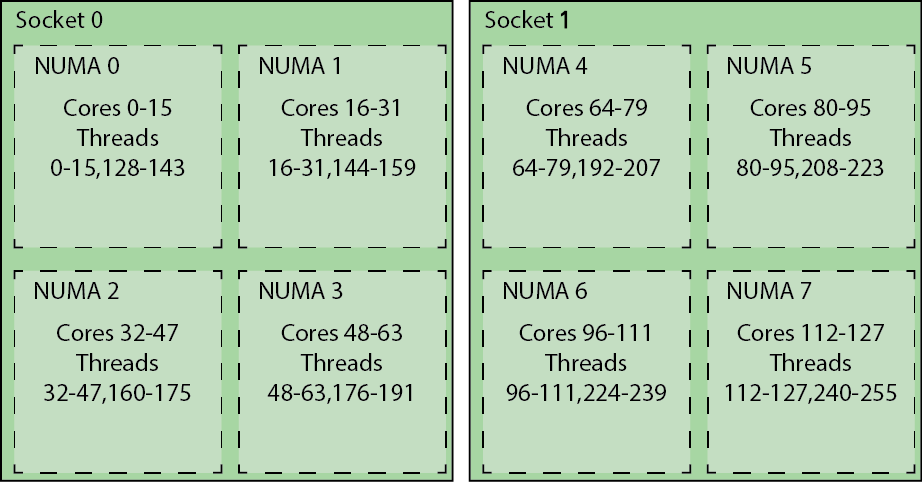
\includegraphics[width=1\textwidth]{figures/mahti_numa.png}
%     \caption{Mahti NUMA structure overview \cite{mahti}}
%     \label{fig_mahti_numa}
% \end{figure}

% Each core possesses 32 KiB of L1 data cache and 32 KiB of L1 instruction cache, and a private 512 KiB L2 cache. Additionally, each core has two FMA (fused multiply-add) units capable of processing operations on full 256-bit vectors. Consequently, each unit can execute operations on eight single-precision floats or four double-precision floats per clock cycle, resulting in 16 double-precision floating point operations per cycle.

% As shown in Figure \ref{fig_mahti_ccd}, cores in the CPU are grouped into core complexes (CCXs) and further combined into compute dies (CCDs). At the CCX level, four cores share a 16 MiB L3 cache within the CCX, and two CCX parts combine to form a compute die (CCD).

% \begin{figure}[H]
%     \centering
%     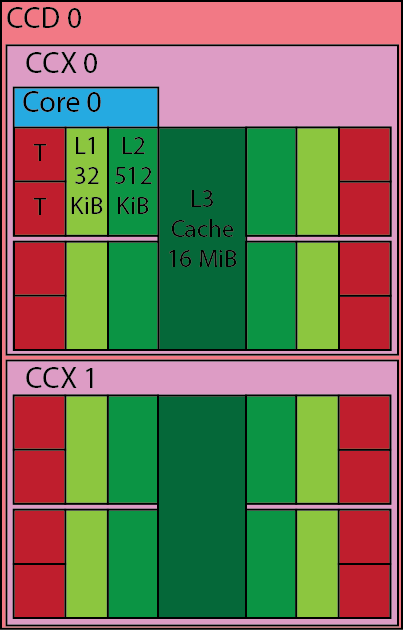
\includegraphics[width=0.3\textwidth]{figures/mahti_ccd.png}
%     \caption{Mahti CCD structure overview \cite{mahti}}
%     \label{fig_mahti_ccd}
% \end{figure}

% Each processor comprises eight compute dies and an additional I/O die, including memory and PCI-e controllers. Furthermore, each node consists of two processors and one 200 Gbps HDR network adapter, as shown in Figure \ref{fig_mahti_node}.

% \begin{figure}[H]
%     \centering
%     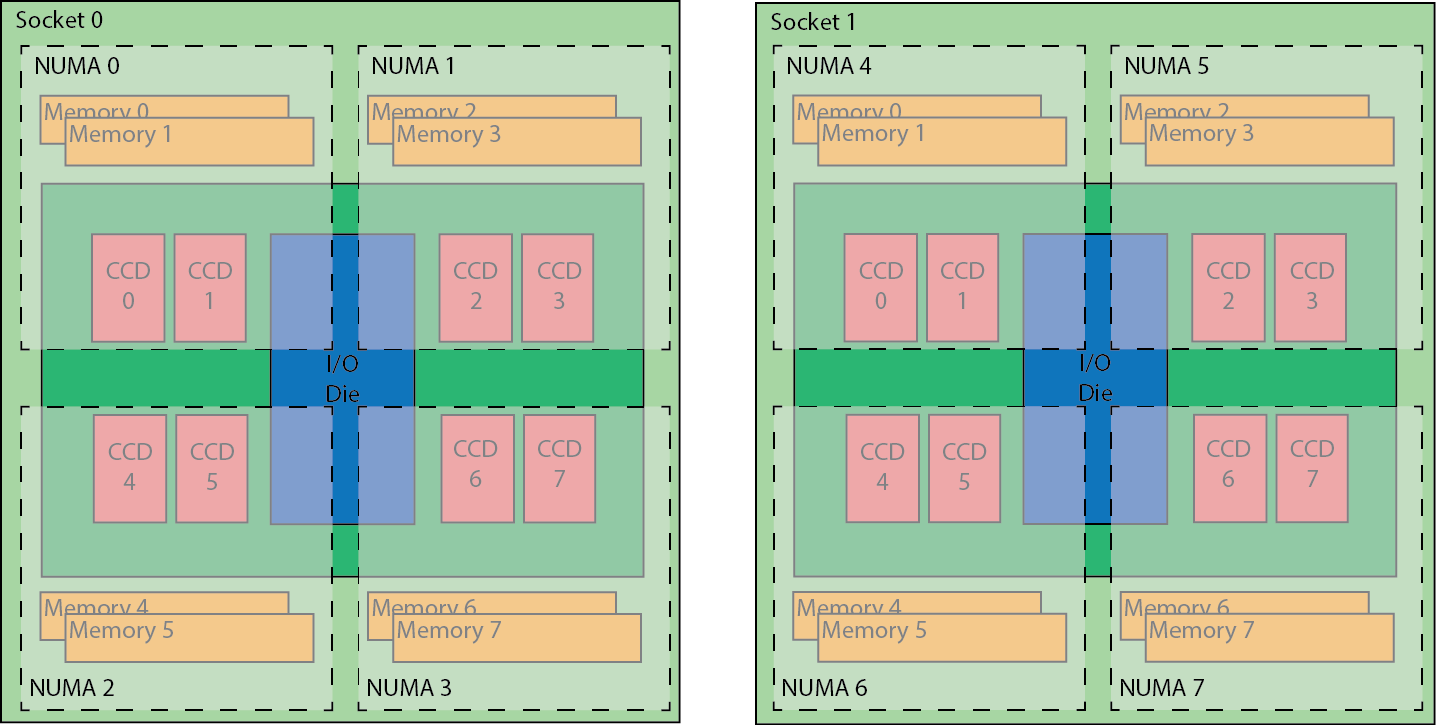
\includegraphics[width=1\textwidth]{figures/mahti_node.png}
%     \caption{Mahti node structure overview \cite{mahti}}
%     \label{fig_mahti_node}
% \end{figure}

% The network interconnect in Mahti is based on Mellanox HDR InfiniBand, with each node connected to the network via a single 200 Gbps HDR link. The network topology adopts a dragonfly+ configuration, wherein multiple groups of nodes are internally connected using a fat tree topology. These fat trees are interconnected using all-to-all links, ensuring fully non-blocking connectivity between groups, as shown in Figure \ref{fig_mahti_df_ex}.

% \begin{figure}[H]
%     \centering
%     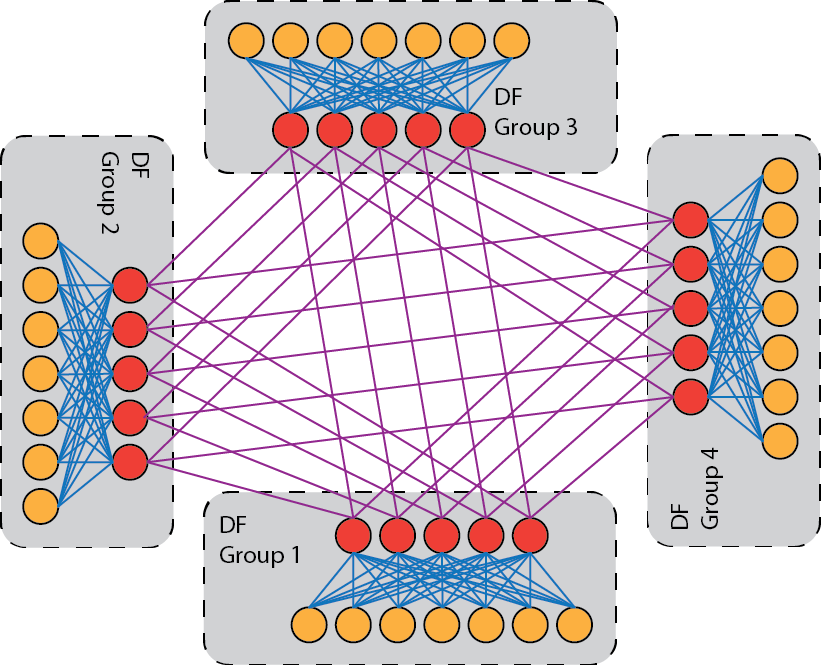
\includegraphics[width=0.6\textwidth]{figures/mahti_df_ex.png}
%     \caption{Mahti dragonfly+ configuration overview \cite{mahti}}
%     \label{fig_mahti_df_ex}
% \end{figure}

% In Mahti, each dragonfly group comprises 234 nodes, with an internal fat tree featuring a blocking factor of 1.7:1 and 20 or 18 nodes connected per leaf switch. Each leaf switch connects to the spine switch in the group via 12 200 Gbps links. Figure \ref{fig_mahti_df} shows the topology of such a group. There are six groups, with five 200 Gbps links connecting each spine switch to a spine switch in every other group, facilitating comprehensive inter-group communication.

% \begin{figure}[H]
%     \centering
%     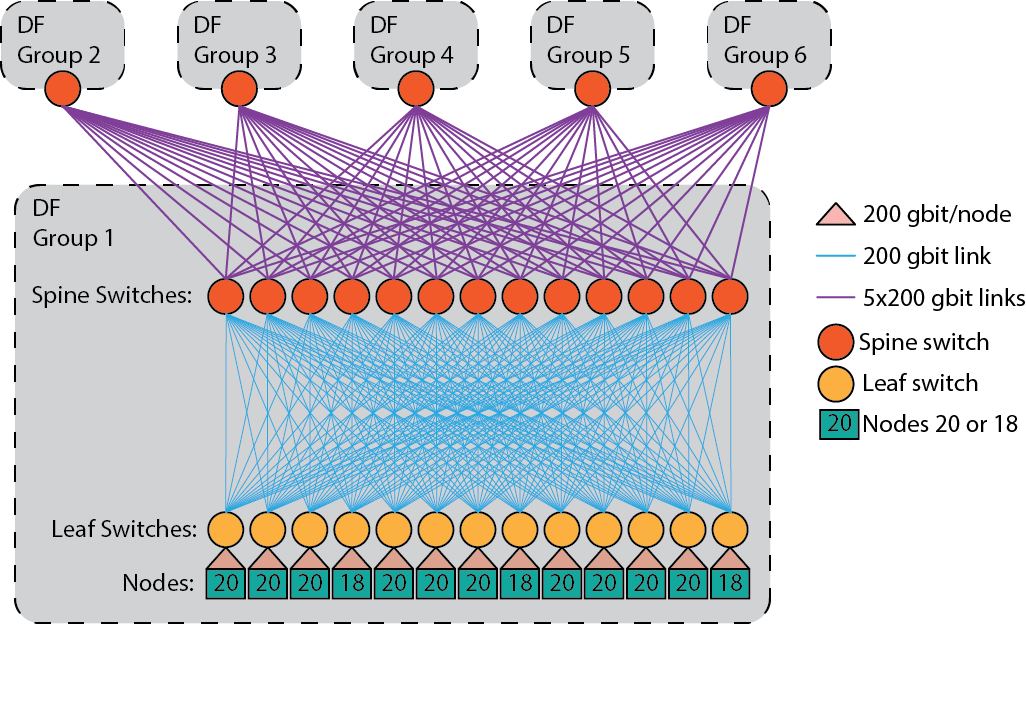
\includegraphics[width=0.8\textwidth]{figures/mahti_df.png}
%     \caption{Mahti dragonfly topology \cite{mahti}}
%     \label{fig_mahti_df}
% \end{figure}

\subsection{LUMI}
\label{subsec:lumi}
By Jun 2024, LUMI \cite{lumi}, one of the three European pre-exascale supercomputers and an HPE Cray EX supercomputer, was the fastest supercomputer in Europe. The GPU partition, LUMI-G, features the primary compute power, which consists of 2978 nodes, as described in Figure \ref{fig_lumig_overview}.

\begin{figure}[H]
    \centering
    \includesvgpath[width=0.9\textwidth]{lumig-overview.svg}
    \caption{LUMI GPU partition overview \cite{lumi}}
    \label{fig_lumig_overview}
\end{figure}

\subsubsection{GPU}

The LUMI-G compute nodes have four AMD MI250X GPUs, each based on the 2nd Gen AMD CDNA architecture. The MI250X GPU is structured as a multi-chip module, which includes two GPU dies referred to as AMD Graphics Compute Dies (GCD). In Slurm and HIP runtime, a single MI250X module is recognized as two GPUs. Thus, in the actual system, the LUMI-G are 8-GPU nodes.

Each GCD has 110 compute units and accesses a 64 GB slice of high-bandwidth memory, totaling 220 compute units and 128 GB of memory per MI250X module. All compute units share an L2 cache with an 8 MB capacity to enhance memory throughput. The cache is divided into 32 slices, capable of delivering 128 B/clock/slice, amounting to a peak theoretical bandwidth of 6.96 TB/s. Including an L2 cache in the MI250X GPU modules enhances synchronization capabilities for algorithms reliant on atomic operations to coordinate communication across the entire GPU. These atomic operations are executed close to the memory within the L2 cache.

% \begin{figure}[H]
%     \centering
%     \includesvgpath[width=1\textwidth]{MI250x-gcd.svg}
%     \caption{AMD MI250X GCD structure \cite{lumi}}
%     \label{mi250x-gcd.svg}
% \end{figure}

% When a kernel is dispatched for execution on the GPU, it is organized as a grid of thread blocks (workgroups), with the grid and thread blocks being one, two, or three-dimensional. The grid can have a maximum number of blocks specified along each dimension of (2147483647, 2147483647, 2147483647), while the maximum number of threads (work-items) for each dimension of a block is (1024, 1024, 1024), with a thread block size limit of 1024, which means size.x * size.y * size.z must be less than or equal to 1024.

% The thread blocks are assigned to one of the 110 compute units and are scheduled in groups of 64 threads known as wavefronts. This is analogous to a warp on NVIDIA hardware, except that a warp consists of 32 threads, while a wavefront comprises 64 threads.

% The execution process of wavefronts by a compute unit can be outlined as follows:

% \begin{enumerate}
%     \item Each wavefront, comprising 64 work items (threads), is allocated to one of the 16-wide SIMD units.
%     \item Most instructions are executed within a single cycle, although one instruction requires four cycles per wavefront.
%     \item With 4 SIMD units available per compute unit, up to 4 wavefronts can be processed simultaneously, ensuring a consistent throughput of one instruction per wavefront per compute unit.
% \end{enumerate}

% Figure \ref{mi250x-compute-unit.svg} shows that each compute unit has 512 64-wide 4-byte vector general-purpose registers. Additionally, the unit provides access to low-latency storage through a 64 kB local data share (LDS, shared memory), accessible to all threads within a block. The programmer manages the LDS allocation. Furthermore, each compute unit has access to 16 kB of L1 cache.

% \begin{figure}[H]
%     \centering
%     \includesvgpath[width=1\textwidth]{mi250x-compute-unit.svg}
%     \caption{AMD MI250X compute unit structure \cite{lumi}}
%     \label{mi250x-compute-unit.svg}
% \end{figure}

% The vector ALUs are complemented by matrix cores optimized to execute matrix fused multiply-add instructions, offering significant acceleration for generalized matrix multiplication computations, crucial for Linear Algebra in High-Performance Computing applications and AI workloads. Each compute unit (CU) has four matrix cores capable of achieving a throughput of 256 double-precision floating-point format (FP64) Flops/cycle/CU.

\subsubsection{CPU}

The CPU of LUMI-G nodes is a 64-core AMD EPYC 7A53 Trento CPU. These CPU cores, built on the Zen 3 architecture, support AVX2 256-bit vector instructions, enabling a maximum throughput of 16 double-precision FLOP/clock (AVX2 FMA operations). Each core has 32 KiB of private L1 cache, a 32 KiB instruction cache, and 512 KiB of L2 cache. The L3 cache has 32 MiB shared among groups of 8 cores, accumulating 256 MiB of L3 cache per CPU. Configured as 4 NUMA nodes (NPS4), the system allocates 128 GiB of DDR4 memory per NUMA node, resulting in 512 GiB of CPU memory.

% \subsubsection{Connections}

% Figure \ref{fig_lumig_topology} shows the node topology. Each MI250X module includes 5 GPU-GPU links, 2 CPU-GPU links, and 1 PCIe link to the slingshot-11 interconnect. The MI250X modules are connected via an in-package Infinity Fabric interface, capable of delivering a theoretical peak bidirectional bandwidth of up to 400 GB/s. Furthermore, GCDs across different MI250X modules are linked through single or double Infinity Fabric links, offering peak bidirectional bandwidths of 100 GB/s and 200 GB/s, respectively. Each MI250X module directly connects to the slingshot-11 network, affording peak bandwidths of up to 25+25 GB/s. 

% \begin{figure}[H]
%     \centering
%     \includesvgpath[width=1\textwidth]{lumig-node-overview.svg}
%     \caption{LUMI GPU node topology overview \cite{lumi}}
%     \label{fig_lumig_topology}
% \end{figure}

% Figure \ref{fig_lumig_cpu_gpu_links} shows the CPU-GPU links from a CPU-centric or GPU-centric point of view of the LUMI GPU node. Proper binding of the NUMA node to the GPU can be essential to ensure optimal application performance.

% \begin{figure}[H]
%     \centering
%     \includesvgpath[width=1\textwidth]{lumig-cpu-gpu-links.svg}
%     \caption{CPU-GPU links on LUMI GPU node \cite{lumi}}
%     \label{fig_lumig_cpu_gpu_links}
% \end{figure}

\section{Monitoring tools}
A robust selection of monitoring techniques is crucial for capturing accurate metrics, diagnosing performance issues, and ensuring efficient resource utilization. This Section explores various components for building a monitoring system, each offering unique capabilities for monitoring within large-scale distributed computing clusters, thus providing the cornerstone for building an accurate alert algorithm.

\subsection{Cgroups}
Cgroups \cite{7876184} is a Linux kernel feature that enables the isolation and accounting of resources, including CPU, memory, and devices, among a collection of processes. It provides a means to track and manage CPU and memory utilization per process.

Slurm can be configured to use Cgroups to regulate resources allocated to jobs, steps, and tasks and for resource accounting. Cgroups have different controllers (subsystems), each responsible for managing specific resources. Slurm's plugins can utilize multiple controllers, including memory, CPU, devices, freezer, cpuset, and cpuacct. Each enabled controller empowers Slurm to enforce resource constraints on a defined set of processes. Slurm cannot enforce resource constraints through Cgroups for the associated resources if a controller is unavailable. Slurm supports two Cgroup modes through plugins: Legacy mode (Cgroups v1) and Unified Mode (Cgroups v2, introduced in Linux Kernel version 5.8).

% Compared with Cgroup v1, Cgroup v2 introduces several enhancements, including:
% \begin{itemize}
%     \item \textbf{Unified Hierarchy Design}: Cgroup v2 adopts a single unified hierarchy structure within the API, simplifying management operations.
%     \item \textbf{Enhanced Container Delegation}: It provides a safer delegation of sub-trees to containers, ensuring improved isolation.
%     \item \textbf{Integration of New Features}: Cgroup v2 incorporates newer features like Pressure Stall Information (PSI), enhancing resource monitoring capabilities.
%     \item \textbf{Improved Resource Management}: It offers refined resource allocation and isolation across multiple resource types, enhancing system performance.
%     \item \textbf{Unified Memory Accounting}: Cgroup v2 uses unified accounting for various memory allocations, including network and kernel memory.
%     \item \textbf{Handling Non-Immediate Resource Changes}: It introduces support for accounting non-immediate resource changes, such as page cache write-backs.
% \end{itemize}

At CSC, Puhti and Mahti still use Red Hat Enterprise Linux (RHEL) 8, which means Cgroup v1. In contrast, LUMI uses a more recent system, SUSE Linux Enterprise Server (SLES) 15 SP4, which means Cgroup v2. So, we need to support both Cgroup versions to cover the CPU and memory monitoring for all the systems.

Cgroups can form the foundation for understanding CPU and memory consumption. Take Cgroups v1, for example:

\begin{itemize}
    \item \textbf{/sys/fs/cgroup/memory/slurm/uid\_*/job\_*/*/memory.usage\_in\_bytes} tells the memory usage for the job.
    \item \textbf{/sys/fs/cgroup/cpuset/slurm/uid\_*/job\_*/cpuset.cpus} tells the list of CPU cores that are used by the job.
\end{itemize}

\subsection{/proc}
The /proc \cite{5544096} directory is unique within the Linux file system, as it functions as a virtual filesystem. Often described as a process information pseudo-file system, it diverges from traditional directories by not containing actual files of the same size since these files serve as pointers, directing users to the underlying location of process information within the kernel. Thus, it provides runtime system data such as system memory utilization, mounted devices, and hardware configurations.

% The /proc serves as a hub for kernel control and information dissemination -- many system utilities directly access files within this directory to gather essential system data. For instance, commands like \texttt{lsmod} and \texttt{lspci} are essentially shorthand for \texttt{cat /proc/modules} and \texttt{cat /proc/pci}, respectively. Furthermore, modifying files within /proc enables users to interact with kernel parameters, facilitating real-time adjustments to system configurations via sysctl.

% A distinctive characteristic of files within /proc is, that they almost all have a file size of 0, with exceptions like kcore, mtrr, and self.

When browsing the directory, we see those numbered subdirectories corresponding to the unique process ID (PID). By cross-referencing these PIDs with the process table, we can identify and examine specific processes. For instance, if the process table denotes a process with PID 1234, accessing the directory /proc/1234 reveals detailed information about this process.
    
The /proc can also form the basis for understanding CPU and memory consumption. Monitoring processes often involve parsing information from /proc to extract consumption-related statistics according to process IDs, including their memory usage and CPU information:

\begin{itemize}
    \item \textbf{/proc/cpuinfo} helps us know the frequency of CPU cores in the current node.
    \item \textbf{/proc/<PID>/status} helps us know how many CPU cores we got allocated, as well as the current Resident Set Size (RSS) and max RSS, which is the maximum amount of memory used at any time by the process in that job context.
    \item \textbf{/proc/<PID>/maps} provides information about memory mappings for the specified process. It includes a list of memory regions allocated to the process and details such as the starting and ending addresses, permissions, and file mappings, if applicable.
\end{itemize}

\subsection{GPU management library}
\subsubsection{NVML}
NVML \cite{nvml} is a GPU-specific library provided by NVIDIA for managing and monitoring NVIDIA GPU devices. Its C-based API is designed to monitor and control the diverse states of NVIDIA GPU devices. This API offers direct access to the queries and commands accessible through Nvidia-SMI. It can help efficiently manage and monitor NVIDIA GPU devices. NVML exposes a comprehensive set of metrics, including GPU temperature, memory usage, and GPU utilization, allowing for detailed insights into GPU performance.

NVML is a cornerstone for GPU monitoring on systems equipped with NVIDIA GPUs, such as Puhti and Mahti.

\subsubsection{ROCm-SMI}
ROCm-SMI \cite{rocm-smi} is an analogous tool to NVML but tailored for AMD GPUs within the Radeon Open Compute ecosystem. Like NVML, ROCm-SMI provides GPU-specific metrics, allowing for the monitoring and managing of AMD GPU devices.

For HPC clusters that utilize AMD GPUs, such as LUMI, integrating ROCm-SMI into the GPU monitoring framework is essential. In contrast, Puhti and Mahti utilize NVIDIA GPUs, so NVML is used in these two systems.

\section{Time-series databases}

% This Section explores two prominent time-series databases, InfluxDB and TimescaleDB \cite{le2021developing}.

% \subsection{InfluxDB}
% InfluxDB is a high-performance, open-source time series database developed by InfluxData. It is written in Go and is optimized for handling time series data at scale, making it a popular choice for use cases involving monitoring performance metrics, IoT data, and real-time analytics.

% InfluxDB is more than just a time series database. It also includes the InfluxDB User Interface (InfluxDB UI) and Flux, a functional scripting and query language that enables sophisticated data transformation.

% InfluxDB 3.0 \cite{10.1007/978-3-031-42529-5_26}, the newest version of InfluxDB, is built in Rust, a modern programming language designed for performance, safety, and memory management. It features a decoupled architecture that allows computing and storage to be scaled independently. InfluxQL is an SQL-like query language that replaces Flux for working with data in InfluxDB databases.

% \subsection{TimescaleDB}
Time-series data management is a critical aspect of data lifecycle management, mainly due to its complexities. Time-series data, comprising a sequence of data points recorded over discrete time intervals, provides invaluable insights into evolving phenomena spanning milliseconds to years. Widely applicable across various domains, time-series data uses time as the principal axis for data organization.

Effectively managing time-series data involves addressing numerous challenges, ranging from efficient data ingestion to optimized query performance and cost-effective resource utilization. Time-series databases play a pivotal role in storing and analyzing time-stamped data efficiently. Choosing the right time-series database is crucial for managing and querying the vast amount of data generated by monitoring metrics, thus contributing to resolving \textbf{RQ1} in Section \ref{sec:rqs}.

One of the primary challenges in time-series monitoring for HPC jobs is handling high cardinality, which refers to the number of unique sets of data combinations. High cardinality can lead to performance bottlenecks as the database needs to manage and index many unique series, each potentially requiring separate storage and processing resources. This can strain the database system's capacity to ingest data rapidly and execute queries efficiently, especially as the data volume scales. Many non-time-series databases, and other time-series databases, including InfluxDB, will crash as the job to record (cardinality) increases.

\subsubsection{TimescaleDB}

TimescaleDB \cite{timescaledb} emerges as a robust solution, excelling in both rapid data ingestion and streamlined query processing, ensuring comprehensive time-series data management capabilities. TimescaleDB is an open-source time-series database optimized for fast ingest and complex queries. It is engineered on top of the mature RDBMS system PostgreSQL and packaged as an extension. TimescaleDB extends PostgreSQL with time-series-specific optimizations and functions, allowing it to manage time series data efficiently. TimescaleDB supports the full range of SQL functionality, including aggregates, joins, subqueries, and window functions.

Central to TimescaleDB's architecture are \textbf{hypertables}, which serve as fundamental structures for efficient time-series data management as shown in Figure \ref{fig:hypertables-chunks}. Hypertables abstract multiple individual tables that store the data, referred to as chunks, providing users with a unified interface for data interaction. With hypertables, users can execute diverse operations, including data insertion, querying, and schema modifications, seamlessly integrating standard SQL functionalities. Hypertables are particularly advantageous for time-series data management, because they efficiently partition incoming data into smaller, manageable subsets. These data subsets, represented as time-based chunks, enable TimescaleDB to handle data retention and optimization efficiently. Consequently, TimescaleDB can do fast data ingestion and is scalable to ions of rows per second, which is crucial for time-series applications.

\begin{figure}[H]
\centering
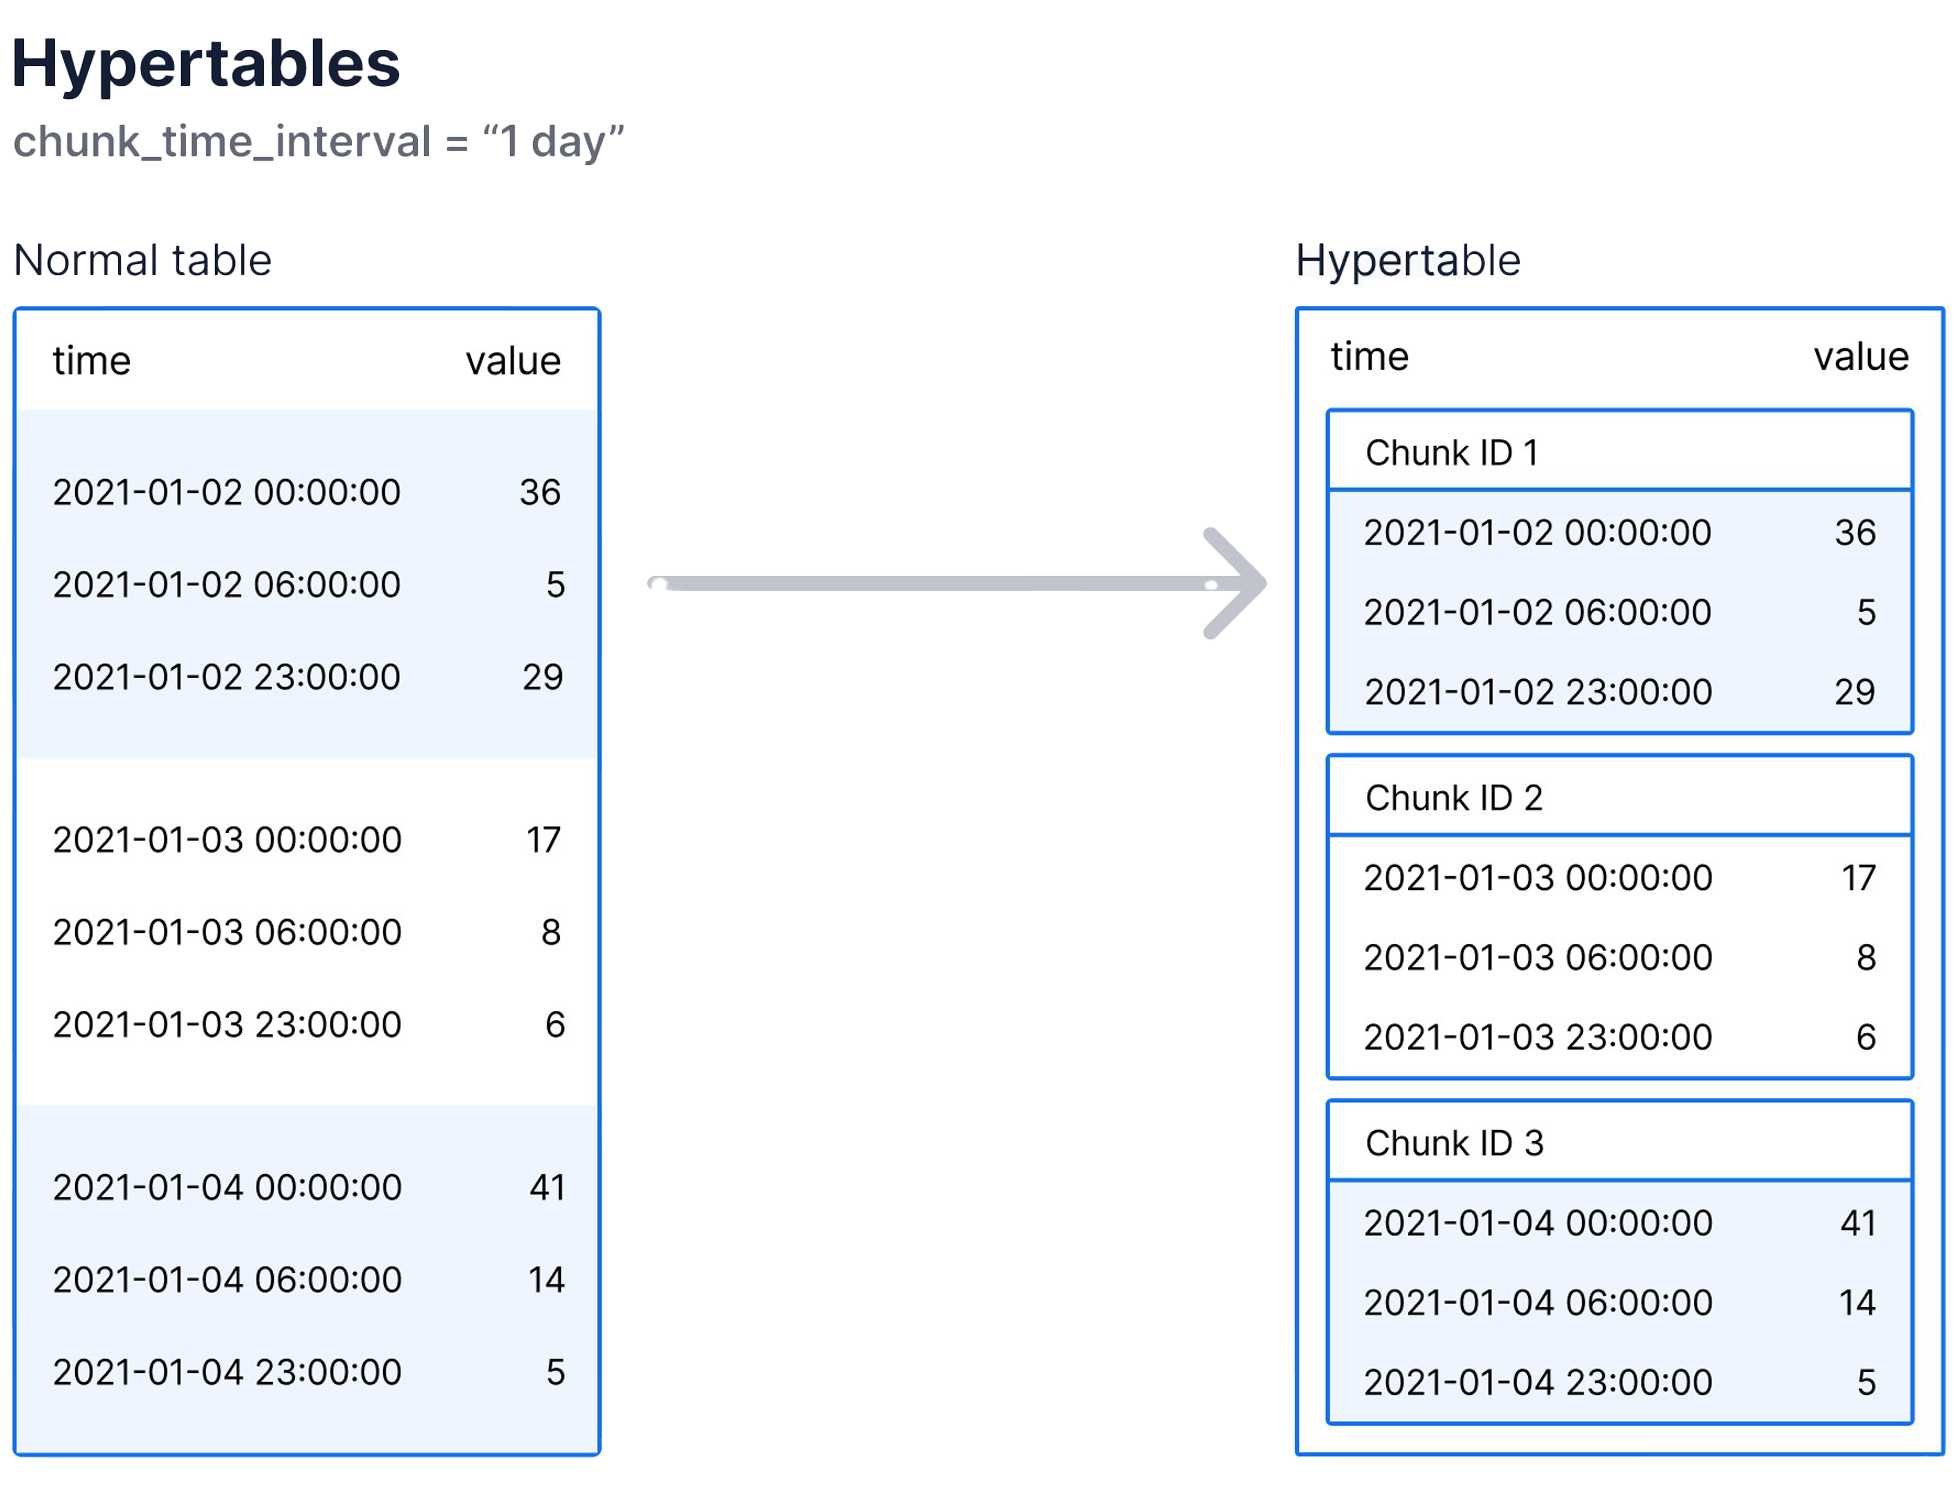
\includegraphics[width=0.9\textwidth]{figures/hypertables-chunks.png}
\caption{Hypertable compared with normal table \cite{hypertables}}
\label{fig:hypertables-chunks}
\end{figure}

Moreover, TimescaleDB effectively addresses cardinality issues. Leveraging hypertables and their automatic partitioning mechanism minimizes the overhead of managing high-cardinality data sets. This partitioning ensures the data is distributed across smaller chunks, reducing the performance impact when querying large datasets and maintaining efficient indexing.

\textbf{Compression} functionalities in TimescaleDB further enhance data storage efficiency. By employing compression algorithms such as delta encoding, delta-of-delta, simple-8b, run-length encoding, etc. \cite{timescaledb-compress}, TimescaleDB significantly reduces disk space utilization, achieving very high compression ratios.

TimescaleDB also facilitates the implementation of \textbf{data retention} policies as background jobs, automating the removal of obsolete data chunks and ensuring efficient data lifecycle management.

These features collectively make TimescaleDB a preferred choice over other time-series databases, especially for applications requiring robust performance under high cardinality conditions.

\section{Database techniques}
Databases are crucial in effectively managing and analyzing time-series data generated in real-time GPU resource monitoring. Our motivation is to create a system that can handle long-term reliable storage and provide near real-time status overviews without heavy SQL searches, thus contributing to resolving both \textbf{RQ1} and \textbf{RQ2} in Section \ref{sec:rqs}. To achieve this, we explore three significant database techniques that can be employed: Triggers, LISTEN \& NOTIFY, and Continuous Aggregates.

\subsection{Triggers}

Triggers \cite{Shaik2023triggers, postgresql-doc} are database elements that automatically respond to specific events or changes in the database. In GPU resource monitoring, a trigger can be activated upon inserting new GPU monitoring data, instantly processing this data and notifying relevant services. This ensures that the data is immediately available for long-term storage and real-time monitoring, facilitating a seamless integration between the two tiers of data management.

% This includes sending notifications via NOTIFY, based on GPU metrics stored in the time-series database.

A trigger in database management serves as a specification, that executes a designated function automatically, whenever a particular type of operation is conducted. The function must be declared as accepting no arguments and returning type triggers. It is important to note, that the trigger function receives input via a specially passed TriggerData structure, rather than conventional function arguments. Triggers can be configured to execute before or after an INSERT, UPDATE, or DELETE operation on a per-row or per-statement basis. Upon occurrence of a trigger event, the designated trigger function is invoked at the appropriate time to handle the event.

PostgreSQL offers two distinct types of triggers: \textbf{per-row (row-level)} triggers and \textbf{per-statement (statement-level)} triggers. Per-row triggers invoke the trigger function once for each row affected by the triggering statement. Conversely, per-statement triggers are invoked only once, when the corresponding statement is executed, irrespective of the number of rows impacted by the statement. Statement-level triggers also lack a mechanism to examine the rows modified by the statement.

Triggers can further be categorized as \textbf{before} triggers or \textbf{after} triggers. Statement-level before triggers are inherently activated before the start of the relevant statement, while statement-level after triggers are triggered upon the end of the statement. On the other hand, row-level before triggers are activated immediately before an operation on a specific row, while row-level after triggers are triggered after the statement but before any statement-level after triggers.

% For per-statement triggers, the trigger functions should, in any case, return NULL. In contrast, trigger functions invoked by per-row triggers can return a table row (a value of type HeapTuple) to the invoking executor. Specifically, a row-level trigger fired before an operation offers the following possibilities:

% \begin{itemize}
%     \item Returning NULL to bypass the operation for the current row, thereby telling the executor to drop the row-level operation that triggered the invocation of the trigger.

%     \item For row-level INSERT and UPDATE triggers exclusively, the returned row assumes the role of the row to be inserted or the row being updated, offering the trigger function the opportunity to modify that row.
% \end{itemize}

% Row-level before triggers, that do not intend to have either of these behaviors must ensure that they return the same row passed in. The return value is disregarded for row-level triggers activated after an operation; hence, they may safely return NULL.

Typically, row-level before triggers are employed for data validation or modification before insertion or updating. Conversely, row-level after triggers are generally utilized to update other tables or perform consistency checks against other tables. This distinction is generated from the fact, that an after trigger can make sure that it is observing the final value of the row, whereas a before trigger cannot. Consequently, if there is no specific rationale for selecting between a before or after the trigger, the before the trigger is preferred for its efficiency, as information about the operation need not be retained until the end of the statement.

% In circumstances where multiple triggers are defined for the same event on a given relation, the related triggers are fired alphabetically by trigger name. In the case of before triggers, the potentially modified row returned by each trigger serves as input to the subsequent trigger. If any before trigger returns NULL, the operation is abandoned for that row, and subsequent triggers are not invoked. Should a trigger function execute SQL commands, these commands may, in turn, trigger additional triggers. This phenomenon, known as \textbf{cascading triggers}, imposes no direct limit on the number of cascade levels. However, trigger programmers must stop infinite recursion from happening in such scenarios.

% During trigger definition, arguments can be specified to facilitate the invocation of different triggers with similar requirements calling the same function. This enables the creation of a generalized trigger function capable of accommodating diverse requirements across multiple tables. The provision of arguments in the trigger definition allows the same function to be leveraged for INSERT events on any table with requisite columns, facilitating automatic tracking of record creation, for instance. Additionally, it can be employed to monitor last-update events if configured as an UPDATE trigger.

The input data within the trigger function includes the trigger event type (e.g., INSERT or UPDATE) and any specified arguments in the CREATE TRIGGER command. For row-level triggers, the input data consists of the NEW row for all types of triggers, and the OLD row for UPDATE and DELETE triggers precisely.

\subsection{LISTEN \& NOTIFY}

LISTEN \& NOTIFY mechanism \cite{Shaik2023listen, postgresql-doc} is a powerful feature in PostgreSQL that provides asynchronous event notification. This technique enables efficient communication between the monitoring infrastructure and other system components, such as the alert service. It helps avoid the overhead of continuous polling and heavy SQL searches, enhancing system efficiency and responsiveness. When a relevant event occurs, such as the arrival of new GPU metrics or job state changes, the NOTIFY command can trigger notifications to any components that have registered interest with the LISTEN command, providing near real-time status updates.

\textbf{LISTEN} command registers the current session as a listener on the notification channel specified by the parameter. All sessions currently listening on the notification channel receive notifications. As a result, each listening session can be notified of its associated client application. Listen registrations of a session are automatically cleared upon the termination of that session.

It is up to the underlying PostgreSQL application programming interface for the client application to detect notification events. For the PostgreSQL driver and toolkit (\textbf{pgx}) package in Golang, listening for notification is a blocking read operation on the underlying socket. It will allocate a connection exclusively for listening purposes, allowing it to be blocked indefinitely.

% For instance, with the libpq library, the application issues LISTEN as a conventional SQL command and periodically calls the PQnotifies function to make sure whether any notification events have been received. 

\textbf{NOTIFY} enables processes accessing a shared PostgreSQL database to exchange information. The data transmitted to the client during a notification event includes the name of the notification channel, the process ID (PID) of the notifying session's server, and the payload string, which defaults to an empty string if unspecified, to client applications previously registered in listening for events on a specified channel within the current database. These notifications are broadcast to all listeners. More complex data structures can be established with database tables, to convey additional information from the notifier to the listeners. 

A practical programming approach to signaling changes to a particular table using NOTIFY involves embedding the NOTIFY command within a trigger, triggered by table insertion.

% It is worth noting that notifications issued within a transaction are only dispatched upon transaction commitment, ensuring consistency in the event of transaction rollback. Notifications received during a transaction are deferred until after completion, to avoid premature delivery in case of a transaction abort.

% Duplicate notifications with identical payload strings within the same transaction deliver only one notification event to listeners. Conversely, notifications with distinct payload strings are treated as distinct events. Additionally, notifications from different transactions are always delivered in the order of transaction commitment, ensuring sequential delivery.

% Implementing LISTEN \& NOTIFY in the monitoring system enhances the responsiveness of the alert service, allowing it to receive notifications about new GPU metrics as they arrive instantly. This approach is precious in scenarios where timely reactions to changes in GPU resource utilization are crucial. By decoupling the notification mechanism from the traditional request-response model via polling, LISTEN \& NOTIFY contributes to the monitoring system's overall efficiency and real-time capabilities.

\subsection{Continuous aggregates}
% Continuous aggregates in TimescaleDB offer a reliable solution for analyzing time-series data trends, leveraging aggregate functions to observe temporal patterns effectively. Unlike traditional approaches, continuous aggregates intelligently update aggregated data, refreshing only relevant portions of chunks based on underlying data modifications. Consequently, continuous aggregates optimize historical query performance while serving as a long-term data repository independent of changes to raw data.

% Continuous Aggregates can contribute to optimizing data storage and query performance. The system can quickly retrieve summarized information for alerting and analysis by pre-computing aggregated values at regular intervals. This approach ensures the monitoring system maintains responsiveness even as the time series data grows, providing administrators with timely insights into GPU resource utilization trends.

Time-series data tends to experience rapid expansion over time. Consequently, aggregating such data into meaningful summaries often encounters considerable latency. Continuous aggregates \cite{10.14778/3611540.3611559} offer a solution by fastening the data aggregation process.

In scenarios where data is collected at high frequencies, it becomes advantageous to aggregate the data into more considerable time intervals, such as minutes or hours. For instance, when GPU usage readings are recorded every second, computing the average GPU usage for each hour means we must scan the entire dataset and recalculate the average with each query execution. There are generally three ways to do the aggregation within TimescaleDB \cite{ConAggs}:

\begin{itemize}
    \item \textbf{Materialized views} is a conventional PostgreSQL feature used for caching the results of complex queries for subsequent reuse. While materialized views do not update regularly, they can be manually refreshed.

    \item \textbf{Continuous aggregates}, exclusive to TimescaleDB, operate similarly to materialized views, but undergo automatic background updates, as new data is appended to the database. These aggregates are continuously and incrementally updated, resulting in lower resource requirements than materialized views. Furthermore, continuous aggregates are compatible with hypertables, and can be queried like standard tables.

    \item \textbf{Real-time aggregates}, another feature unique to TimescaleDB, share similarities with continuous aggregates. However, incorporate the latest raw data with previously aggregated data, to deliver accurate and up-to-date results without necessitating real-time data aggregation.
\end{itemize}

Continuous aggregates represent a materialized view that undergoes automatic refresh in the background, as new data is introduced or existing data is modified. These aggregates effectively track alterations to the dataset, ensuring the underlying hypertable is consistently updated. Furthermore, the maintenance overhead associated with continuous aggregates is substantially lower than conventional PostgreSQL materialized views. This efficiency allows users to focus on data analysis, rather than database maintenance.

% Given their basis on hypertables, continuous aggregates are queried in the same manner as standard tables. Additionally, users can implement compression or tiered storage configurations on their continuous aggregates. Moreover, continuous aggregates can be nested, enabling the creation of aggregates on top of existing aggregates.

Continuous aggregates comprise the following components:

\begin{itemize}
    \item \textbf{Materialization hypertable}: The intermediary repository for aggregated data, which is retrieved as required. It consists of columns representing various group-by clauses in the query, a chunk column identifying the corresponding data chunk, and partial aggregate columns for each aggregate function specified in the query. The partial columns are crucial in aggregating data across chunks, particularly when groups span multiple chunks.

    \item \textbf{Materialization engine}: Responsible for orchestrating two transactions— the first determines the time range for materialization and updates the invalidation threshold. In contrast, the second executes the actual materialization process. Notably, most work occurs during the second transaction to prevent interference with other operations.

    \item \textbf{Invalidation engine}: Monitors changes to data in the hypertable and ensures timely re-materialization of affected rows. The invalidation prioritizes recent changes to minimize performance overhead.

    \item \textbf{Query engine}: Allows access to aggregated data in materialization hypertable.
\end{itemize}

For real-time continuous aggregates, it provides data by combining pre-aggregated data from materialized views with recent unaggregated data, ensuring that query results remain up-to-date.

% \section{Event stream management}
% Event Stream Management involves ingesting, analyzing, and storing streams of events, which are discrete data points denoting state changes. This allows for real-time analytics and decision-making. In this Section, we explore some of the state-of-the-art open-source event stream management platforms to give an overview.

% \begin{itemize}
%     \item \textbf{MapReduce} \cite{hashem2016mapreduce} is a programming model for processing large data sets with a parallel, distributed algorithm on a cluster. A MapReduce program comprises a map procedure, which performs filtering and sorting, and a reduce method, which performs a summary operation. The MapReduce algorithm contains two important tasks, namely Map and Reduce. The map script takes some input data and maps it to \texttt{<key, value>} pairs according to the specifications. The reduce script takes a collection of \texttt{<key, value>} pairs and "reduces" them according to the specifications. MapReduce is primarily used for batch processing of large datasets and is not designed for real-time processing or low-latency queries.

%     \item \textbf{Apache Spark} \cite{10.1145/2783258.2789993} is an open-source cluster-computing framework. It provides elegant development APIs for Scala, Java, Python, and R that allow developers to execute a variety of data-intensive workloads across diverse data sources, including HDFS, Cassandra, HBase, S3, etc. Spark provides a faster and more general data processing platform. Spark lets users run programs up to 100x faster in memory or 10x faster on disk than Hadoop. Spark's versatility makes it suitable for various applications and industries.

%     \item \textbf{Apache Flink} \cite{10.14778/3137765.3137777} is a Big Data processing framework that allows programmers to process vast data efficiently and in a scalable. Flink primarily focuses on real-time stream processing, efficiently processing large volumes of data with low latency. Flink's processing engine is built on top of its streaming runtime and can handle batch processing. Flink provides robust Java, Scala, and Python APIs for developing data processing applications.

%     \item \textbf{Apache Kafka} \cite{10213406} \textbf{/ Apache Pulsar} \cite{Sharma2022pulsar} is a real-time event-streaming platform that collects, stores, and processes messages. It provides excellent performance, too, at scale. On top of that, it provides capabilities such as stream processing, distributed logging, and pub-sub messaging. An event (or message) in Kafka consists of Key and Value.
% \end{itemize}

% All four technologies can handle big data, but each has strengths and ideal use cases.

% \begin{itemize}
%     \item MapReduce is primarily used for batch processing of large datasets. It is not designed for real-time processing or low-latency queries.
%     \item Apache Spark, on the other hand, while initially designed for batch processing, has evolved to handle real-time data processing through micro-batching.
%     \item However, Apache Flink was designed as a stream-first framework, excelling in real-time stream processing. It efficiently processes large volumes of data with low latency.
%     \item Apache Kafka, similar to Flink, is designed for real-time data streaming. However, Kafka is more focused on the messaging system, providing a robust platform for storing, reading, and analyzing streaming data.
%     \item Apache Pulsar combines the strengths of both a message queue system and a streaming platform, making it a versatile choice for many use cases.
% \end{itemize}

% \section{Streaming analytics}

% \subsection{Google Datastream}
% Google Datastream is a serverless and easy-to-use change data capture (CDC) and replication service that lets us synchronize data reliably and with minimal latency. It provides seamless replication of data from operational databases into BigQuery. Datastream supports Oracle, MySQL, and PostgreSQL sources. It enables near real-time insights in BigQuery and offers streamlined integration with Dataflow templates to build custom workflows for loading data into a wide range of destinations.

% \subsection{Google BigQuery}
% Google BigQuery is a fully managed enterprise data warehouse that helps manage and analyze data with built-in features like machine learning, geospatial analysis, and business intelligence. BigQuery's serverless architecture lets us use SQL queries to answer the organization's biggest questions with zero infrastructure management. BigQuery's scalable, distributed analysis engine lets us query terabytes in seconds and petabytes in minutes.

% \subsection{Azure Stream Analytics}
% Azure Stream Analytics is a fully managed stream processing engine designed to analyze and process large volumes of streaming data with sub-millisecond latencies. We can build a streaming data pipeline using Stream Analytics to identify patterns and relationships in data that originate from various input sources. Azure Stream Analytics is also available on the Azure IoT Edge runtime, which enables us to process data directly from IoT devices.

% \subsection{Amazon Kinesis}
% Amazon Kinesis cost-effectively processes and analyzes streaming data at any scale as a fully managed service. With Kinesis, we can ingest real-time data, such as video, audio, application logs, website clickstreams, and IoT telemetry data, for machine learning (ML), analytics, and other applications. Amazon Kinesis Data Streams is a serverless streaming service that simplifies capturing, processing, and storing data streams at any scale.

% \subsection{Kapacitor}
% Kapacitor is an open-source data processing framework that makes it easy to create alerts, run ETL jobs, and detect anomalies. Kapacitor tasks define work to do on a data set using TICKscript syntax. Kapacitor tasks include stream tasks, which replicate data written to InfluxDB in Kapacitor, offloading query overhead and requiring Kapacitor to store the data on disk, and batch tasks, which query and process data for a specified interval.

\section{Alert algorithms}
This Section explores the alert algorithms we can use, including descriptive statistics, decision trees, random forest, and K-Means clustering, thus trying to resolve \textbf{RQ4} in Section \ref{sec:rqs}. Although deep learning models are powerful tools with great flexibility and capacity to learn feature hierarchies from raw data, they come with challenges. They can hardly be used in our case, since they require a large amount of data and substantial computational resources, which makes them less efficient compared to simpler models like decision trees and random forests when dealing with smaller datasets or when computational resources are limited. Furthermore, deep learning models can be challenging to interpret and require careful tuning to avoid over-fitting.

\subsection{Descriptive statistics}
\label{subsec:statistics}
Descriptive statistics is a branch of statistics that summarizes the data through numerical calculations. Its main purpose is to simplify and present data in an easy-to-understand format. Key measures include:

\begin{itemize}
\item \textbf{Central Tendency:} Mean, median, and mode. These measures of central tendency describe a distribution's center position.
\item \textbf{Dispersion:} Standard deviation, range, variance, and interquartile range. These are measures of dispersion that describe the spread of data.
\item \textbf{Skewness and Kurtosis:} These are measures of shape that describe the asymmetry and peakedness of a distribution, respectively.
\end{itemize}

Here is a list of definitions of these possible descriptive statistics:

\begin{itemize}
    \item \textbf{Percentiles (25\%, 50\%, 75\%)}: Statistical measures used to describe the distribution of a dataset. The 25th, 50th, and 75th percentiles are commonly known as the first quartile (Q1), median, and third quartile (Q3) respectively. They represent the values below which a given percentage of observations fall.

\[
\text{{Percentile}}(X, p) = \text{{value below which }} p\% \text{{ of the data fall}}
\]

    \item \textbf{Kurtosis}: Measure of the \textit{tailedness} or \textit{sharpness} of the peak of a distribution. Positive kurtosis indicates a sharper peak (leptokurtic), while negative kurtosis indicates a flatter peak (platykurtic). The formula for kurtosis is given by:

\[
\text{{Kurtosis}}(X) = \frac{n(n+1)}{(n-1)(n-2)(n-3)} \sum_{i=1}^{n} \left(\frac{X_i - \bar{X}}{s}\right)^4 - \frac{3(n-1)^2}{(n-2)(n-3)}
\]

    \item \textbf{Maximum}: The highest value in a dataset, which is the extreme upper end of the distribution.

    \item \textbf{Mean}: The average of all values in the dataset and is calculated as:

\[
\text{{Mean}}(X) = \frac{1}{n} \sum_{i=1}^{n} X_i
\]

    \item \textbf{Minimum}: The lowest value in a dataset represents the distribution's extreme lower end.

    \item \textbf{Skewness}: The asymmetry of a distribution. Positive skewness indicates a longer right tail, while negative skewness indicates a longer left tail. The formula for sample skewness is given by:

\[
\text{{Skewness}}(X) = \frac{n}{(n-1)(n-2)} \sum_{i=1}^{n} \left(\frac{X_i - \bar{X}}{s}\right)^3
\]

    \item \textbf{Variance}: Measure the average squared deviation of each data point from the mean. The formula for sample variance is given by:

\[
\text{{Variance}}(X) = \frac{1}{n-1} \sum_{i=1}^{n} (X_i - \bar{X})^2
\]

    \item \textbf{Standard Deviation}: Measure the variation or dispersion in a dataset. It is calculated as the square root of the variance:

\[
\text{{Standard Deviation}}(X) = \sqrt{\text{{Variance}}(X)}
\]


\end{itemize}

\subsection{Decision tree}

A decision tree \cite{song2015decision} represents possible solutions to a decision based on branches of certain conditions and reaches several conclusions based on the conditions. As shown in Figure \ref{fig_decision_tree}, the main components of a decision tree are:

\begin{itemize}
\item \textbf{Root Node:} Collection of all the data that can be divided into two or more homogeneous sets.
\item \textbf{Splitting:} The process of dividing a parent node into two or more sub-nodes.
\item \textbf{Decision Node:} The split sub-nodes.
\item \textbf{Leaf Node:} Terminal nodes that do not further split.
\end{itemize}

\begin{figure}[H]
    \centering
    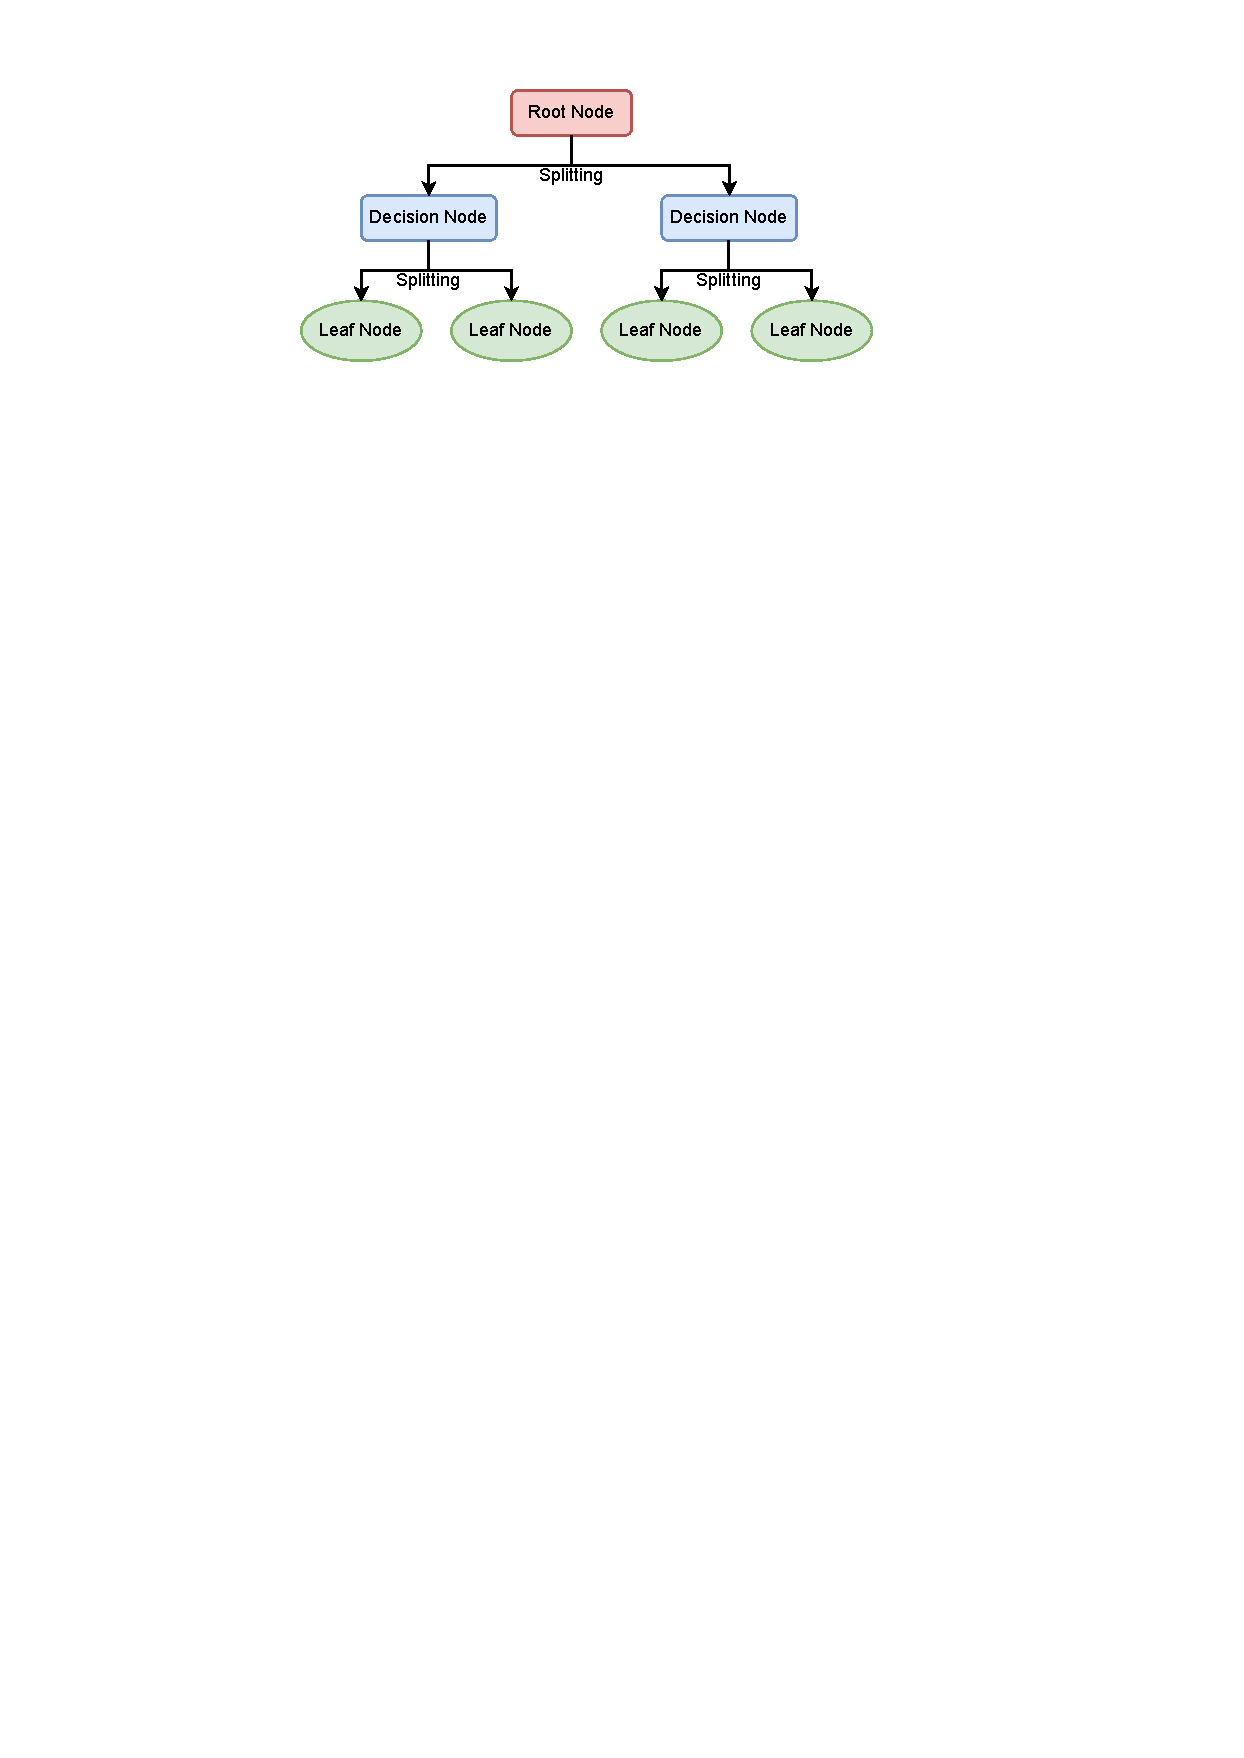
\includegraphics[width=0.6\textwidth]{figures/decision-tree.pdf}
    \caption{Decision tree structure}
    \label{fig_decision_tree}
\end{figure}

\subsection{Random forest}

Random forest \cite{598994} is an ensemble machine learning algorithm with many individual decision trees. Each tree in the random forest gives a prediction, of which the model's final prediction is the most voted class.

Extremely Randomized Trees (or Extra Trees) \cite{geurts2006extremely} is a type of ensemble learning technique that aggregates the results of multiple de-correlated decision trees to reach its final result. The fundamental difference between random forests and extra trees is selecting the cut points to create the decision trees. Extra Trees selects these cut-points comprehensively at random, while traditional decision tree-based algorithms (like Random Forest) select the optimal ones.

\subsection{K-Means clustering and silhouette analysis}
\label{subsec:silhouette}

K-means clustering \cite{Wu2012} is a linear clustering method widely used in data mining and machine learning that aims to partition data into several linearly separable homogeneous groups. It is an unsupervised learning method, meaning a training set is not required, making it more sensible for unlabelled data.

Silhouette analysis \cite{10.1007/978-3-319-62416-7_21} is an unsupervised method used for performance evaluation in machine learning for clustering algorithms such as k-means clustering, which examines the separation distance among resulting clusters and offers a visual means to evaluate parameters such as the number of clusters. The silhouette index in the plot effectively illustrates the proximity of each point within one cluster to points in neighboring clusters that fall within the range of [-1, 1].

Silhouette coefficients close to +1 imply that a sample is far from neighboring clusters, which means good separation. A value of 0 suggests the sample data is on or near the decision boundary between two adjacent clusters. In contrast, negative values imply the possibly wrong classification of a cluster. Furthermore, the thickness of the silhouette plot allows for the visualization of cluster sizes.

% Silhouette analysis can be used to evaluate the validity of the clustering results. It can be compared with the K-means cost function and the original silhouette to find the best way to automate the selection of the best clustering result from a set of K-means clusterings with different parameter configurations.

\section{Summary}
In this Section, we have delved into the intricacies of designing and implementing a real-time GPU monitoring and alerting system for large-scale distributed computing environments, focusing mainly on HPC clusters. By leveraging monitoring techniques, database technologies, and event stream management platforms, we aimed to address the need for efficient resource utilization and performance monitoring in these complex computing infrastructures.

The exploration began with an overview of Slurm, emphasizing its role in resource allocation, job scheduling, and management.

Subsequently, we provided insights into the architecture and specifications of three HPC systems at the CSC-IT Center for Science: Puhti, Mahti, and LUMI. These systems represent state-of-the-art computing clusters with diverse GPU configurations, highlighting the need for a flexible and scalable monitoring solution to accommodate varying hardware architectures.

We then delved into monitoring systems, exploring essential techniques and tools such as /proc, Cgroups, NVML, and ROCm-SMI for capturing resource utilization metrics at both the CPU and GPU levels. Additionally, we discussed the significance of time-series databases like TimescaleDB and related techniques such as triggers, LISTEN \& NOTIFY, and continuous aggregates in efficiently storing and querying monitoring data, enabling real-time analysis and visualization.

% Event stream management platforms such as MapReduce, Apache Spark, Apache Flink, and Apache Kafka/Pulsar were also examined, offering insights into their capabilities and ideal use cases for real-time data processing and analytics.

Finally, we explored various alert algorithms, including descriptive statistics, K-means clustering, silhouette analysis, decision trees, and random forests, as potential methods for identifying patterns or anomalies necessary to catch attention.
